\documentclass[11pt,a4paper]{article}
\usepackage[utf8]{inputenc}
\usepackage[T1]{fontenc}
%\usepackage{gentium}
\usepackage{mathptmx} % Use Times Font

\usepackage{graphicx} % Required for including pictures
\usepackage{hyperref} % Format links for pdf
\usepackage{biblatex}
\addbibresource{references.bib}
\usepackage{booktabs} % Used so that tables generated by pandas
                      % to_latex() work correctly

\frenchspacing % No double spacing between sentences
\usepackage[margin=1in]{geometry}

\usepackage[all]{nowidow} % Tries to remove widows
\usepackage[protrusion=true,expansion=true]{microtype} % Improves typography, load after fontpackage is selected

\usepackage{lipsum} % Used for inserting dummy 'Lorem ipsum' text into the template
\usepackage{float}
\title{Performance of Scottish A\&E services}

\begin{document}

\maketitle

\section{Overview}
The health and well-being of its people is one of the biggest interests of a nation. The time required to provide necessary care in cases of emergency dictates a patient's life. This report accesses the Performance of Scottish A\&E (short for Accident and Emergency) services using the 4-hour waiting time standard performance measure. Public Health Scotland has collected data on the attendance of patients to facilities across the country, the type of care received and compliance with the 4-hour standard.

The data set was first cleaned by removing all the Episodic data, discharge locations and other less useful information. The cleaned data was used for visualisations like monthly compliance\% (to 4-hour standard) aggregated across all the counties, Change in compliance\% of different NHS regions which included pre and post COVID-19 pandemic months. A plot between number of attendances in a month and compliance was also made. Statistical models like Linear Regression was used to spot overall trend.

Our Visualisations show inverse proportionality between the Number of Attendances in a month and the compliance percentage achieved by the Treatment Location, i.e. if there is more crowding in the department, then the compliance percentage will be low. The Attendance plot shows that during lockdown, the patient number, along with the compliance percentage, decreased by a significant amount. Figure 4 shows that boards with less population under them, like NHS Western Isles, had less problem in achieving 95\% compliance than bigger boards like NHS Lothian and NHS Greater Glasgow and Clyde.

%Our assessments include examination of Compliance Percentage of Scottish services to this standard, observing changes in compliance over time and discussing about the events that have caused these changes.

%The study uses the data collected by the Public Health Scotland which is Scotland’s lead national agency for improving and protecting the health and well being of all of Scotland’s people. The Data was cleaned and grouped on a monthly basis.

\section{Introduction}

\paragraph{Context and motivation}
The 4-hour standard implies that no patient should spend longer than 4 hours between arriving at the A\&E unit and admission, discharge or transfer, unless there are stated clinical reasons for keeping the patient in the unit the\cite{ISD_scotland_home}.This standard came after the English Government in 2004 introduced a rule that 98\% of patients will spend no longer than 4 hours in the emergency department; which then was adopted by nations in the British isles including Scotland\cite{NHE}. Since 2007, Scotland's A\&E standard is only valid onto new and unplanned attendances to the A\&E service, so any appointed visit to this department may not abide by this rule.

The regular and correct reporting of such measures helps government bodies like the NHS in the allotment of resources across the country and enables us to access government efforts to improve the country's health care services. Patients spending more time in the emergency department will lead to commotion and this causes patient morbidity and even mortality as a lot of the case are time sensitive. This study tries to further investigate into this. 


\paragraph{Previous work}

Higginson et al. \cite{higginson} demonstrates the correlation between ED crowding and performance against the 4-h standard. But this study has used data from England.  

Public Health Scotland \cite{waiting_time_publication} use the same statistics in their report on A\&E waiting times where they compare compliance percentage of different boards, monthly compliance in the department and Destination on leaving the department. This is closely related to our report. They are not using any statistical methods or deriving any inference from the compiled data.

Sushrut Oomman et al. \cite{Oomman48} demonstrated the performance of A\&E before and during the lockdown using the data collected by County Durham and Darlington NHS Foundation Trust (CDDFT)\cite{CDDFT} and concluded that fear of catching covid-19 in the hospital environment made people reluctant to visit the hospital. 
%Brief description of any previous work in this area (e.g., in the
%media, or scientific literature or blogs).

\paragraph{Objectives}

We would like to answer few questions like: 

How well have services complied with 4-h waiting time standard?

What impact did COVID-19 pandemic had on Number of Attendances and compliance to the standard?

Which NHS regions were worst effected due to the pandemic and what were some possible reasons for it?

Does the activity at some treatment locations change more than others over time?

Was there any change in compliance percentage between 2007 and 2020 (pre-pandemic times only)?

\section{Data}
% Suggested 300 words

\paragraph{Data provenance} 

The Dataset used for this report was created by Public Health Scotland\cite{PHS} which is Scotland's lead national agency for improving and protecting the health and well being of all of Scotland’s people. The agency provides the data with key statistics of attendances at A\&E services across Scotland; They provide data to download for free from their website\cite{waiting_time_publication}, this data was published on 1st Febuary 2022 and it includes records up til Dec 2021. All the publications from Public Health Scotland are made available under the Open Government License \cite{open_government_licence} \cite{permission} which allows us (among other rights) to copy, publish, distribute and exploit the information.


\paragraph{Data description} 

The Scottish A\&E records dataset was formatted as a .csv file containing 15471 records and 17 columns dating from July 2007 to December 2021. Each record contained the information of A\&E attendances and discharges for a Treatment Location over a calendar month. 
This report mainly focuses on the following columns-
\begin{itemize}
    \item Data\_Month\_Date - Stores the month and year of the record.
    \item HB\_Treatment\_Description - stores the NHS board of the record
    \item Number\_Of\_Attendances\_agg \& Number\_Meeting\_Target\_agg - stores total number of attendances and number of attendances meeting 4-hour target respectively. They are used to calculate compliance percentage.
\end{itemize}

There are 13 more columns in the table which are not used in this report, their description is provided in "A\&E activity waiting times statistics.csv" which can be downloaded under open government license from PHS website \cite{waiting_time_publication}


\paragraph{Data processing} 
The data from the csv file was converted to a pandas dataframe inside the jupyter notebook. All the columns mentioned above as used were kept and rest of them were dropped to form a new DataFrame. Dataframe was cleaned by replacing all the NaN values with 0. This dataframe was then made into 3 different dataframes by grouping the records by -
\begin{itemize}
    \item NHS board: summing all the records of a board into single record. We got one record each for all 14 boards. 
    \item Month-Year of the record: summing the records of all the boards with same month and year. We got records starting from July 2007 to December 2021.
    \item NHS board and Month-Year: In this we sum all the records with a particular board for a particular month-year.
\end{itemize}
Compliance Percentage was calculated for each records in these dataframes using the equation:
\begin{equation}
    (Number\_Meeting\_Target\_agg - Number\_Of\_Attendances\_agg) /100
\end{equation}
A new column called 'compliance' : stores the compliance percentage; was appended.

\section{Exploration and  analysis}

\subsection{Visualisations}

\begin{figure}[h]
  \centering
  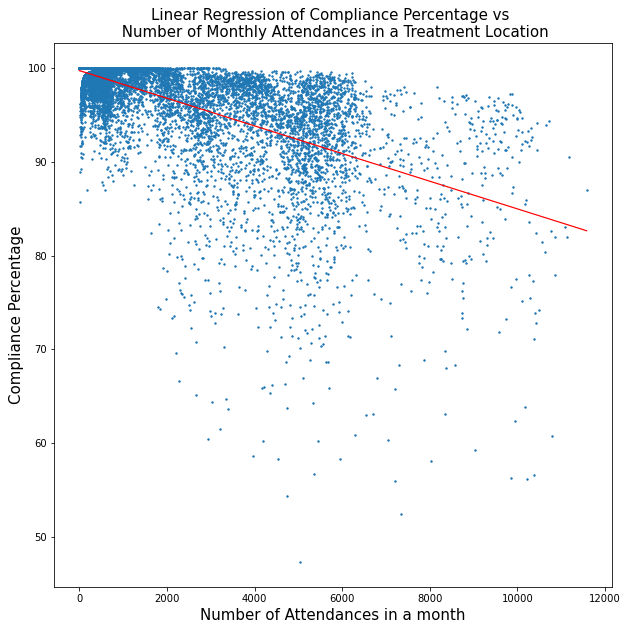
\includegraphics[width=0.8\linewidth,height = 100mm]{regression_attendances_compliance.png}
  \caption{Linear Regression plot.}
\end{figure}


\begin{figure}[h]
  \centering
  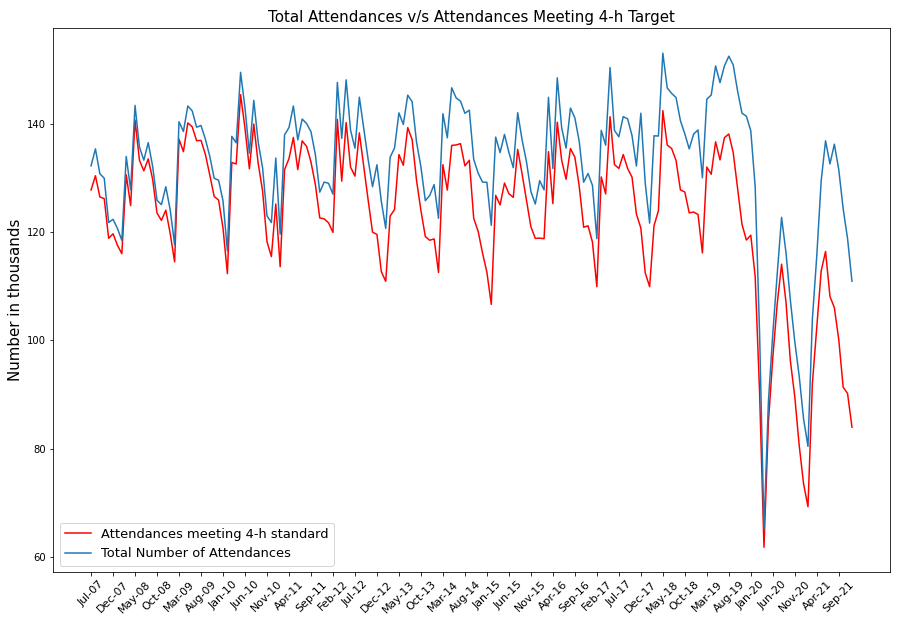
\includegraphics[width=0.8\linewidth]{total_meeting_target.png}
  \caption{Attendance plot}
\end{figure}

\begin{figure}[h]
  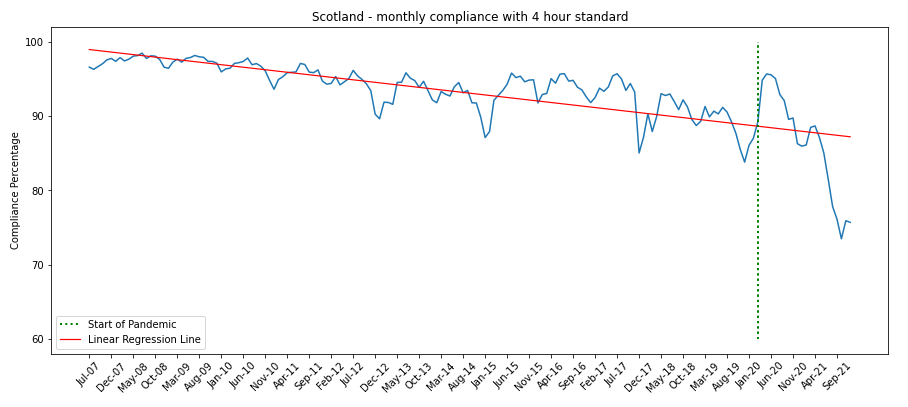
\includegraphics[width=\linewidth]{monthly_compliance_with_4_hour_standard.png}
  \caption{Scotland Monthly Compliance plot}
\end{figure}


\subsection{Interpretation of the results}
Figure 1: shows the plot between Total Number of Attendances and Compliance Percentage, the plot shows clustered high compliance points when number of patients is low and more spread out and low compliance when dealing with huge patient groups. One can also deduce the difference in performance of various treatment locations, as some can handle larger volumes of patients and still meet the 98\% compliance, whereas others struggle even for smaller volumes of attendance.

Figure 2: We have seen that compliance with the 4-hour standard decreased with the onset of the pandemic, but this figure also shows that total attendance to the A&E has also decreased. This is due to measures like lockdown and self-isolation taken in response to the spread of the disease. We observe that since summer 2021, attendance has again started to rise to pre-pandemic numbers.

Figure 3: shows the compliance percentage of all the NHS boards summed every month. There has been a gradual decrease in compliance over the years, with some sudden dips around the December months. This could be due to the holiday season, but no significant evidence supports this claim. Nevertheless, we observe a steep decline in compliance rate after the start of COVID-19 pandemic. This could have been caused by strict isolation and critical care needed for a patient in the A\&E department who the SARS-COV-2 virus has infected. Compliance fell below 80 per cent in the summer of 2020 and has stayed there for almost 1.5 years.

Figure 4: This figure tries to find the regions that were most affected during the pandemic, which could help the NHS improve its services in these regions. Western Isles, Orkney, Tayside, Shetland, and Highlands are the least effected regions, with consistent compliance rates over time. Lanarkshire, Lothian, Forth Valley, and Borders were the most affected regions, with percentages going below 70 per cent.

\subsection{Application of statistical methods(s)}

The Performance of A\&E service location will depend on the total number of patients who visit the department in a month, so it is fitting to use Linear Regression to obtain a regression line. If we estimate the number of attendances, we can predict the locations' performance and improve services where needed. The statsmodels library was used to create and fit the data onto a Linear regression model using the Least Squares method, the ungrouped data was used here which has 15471 datapoints. 

\subsection{Interpretation of the findings}

The built-in summary function from stats models was used to calculate the coefficient of determination $R^2$ for Goodness-of-fit. $R^2$ value of 0.427 was reported which may be interpreted as a bad fit for the given data; but because human diseases and recovery are governed by various factors of which very few were taken in account, greater amounts of unexplainable variation was to be expected. A High F-statistic value of $1.152 * 10^4$ also suggests a goot fitting for the data.



\section{Discussion and conclusions}
% Suggested 400 words.

\paragraph{Summary of findings}
Overall number of attendances to the A\&E service had decreased during the covid-19 lockdown, but it has started to climb back to its normal levels. We expect that if attendance went down, compliance should go up, but during the pandemic, the compliance was low even with low turnout on the A\&E. Some regions were better in adapting changes and hence most people from these regions received care within the standard 4-hour period.

\paragraph{Evaluation of own work: strengths and limitations}
One of the strengths of this report is the visualisations which are clear enough and answer all the questions that we set out to answer.
The linear regression model was one of the limitations of this report, as a better fit could have been made if some outliers had been omitted from the data.

Since the compliance percentage also depended on Treatment location, using some form of multiple regression techniques would have been better. Our Regression line is monotonically going downwards, which hides the fact that compliance percentages are climbing back to their pre-pandemic levels starting from 2021.
Other confounding variables like socio-economic deprivation of that area might also effect the care provided to the patients, not including these is also a limitation to our report.

\paragraph{Comparison with any other related work}
Higginson et al. \cite{higginson} used bed occupancy as a dependant varible to the 4-hour compliance, this is slightly different from Number of attendances that we used as not all patients in the A\&E will require beds during their stay in the department.

Our conclusion and visualisation were really close to the report published by Public Health Scotland, as we used the same dataset for our inference.

We reasoned that reduction in number of attendances during the pandemic due to measures taken by government to stop the spread. Sushrut Oomman et al. \cite{Oomman48} had a different conclusion that it was fear of catching COVID-19 that discouraged people from going to the hospital


\paragraph{Improvements and extensions}
As mentioned above, the regression line in Figure 1 can definitely be improved by deploying multiple regression techniques to better predict the data.

We can extend this report by using different databases like the Scottish Index of Multiple Deprivation\cite{SIMD}, which includes the socio-economic background of the area and thus might be able to better explain the compliance percentage we got from that area. For example, a less deprived area might have bigger budgets for the A\&E services and thus perform better than more deprived areas.

\begin{figure}[H]
  \centering
  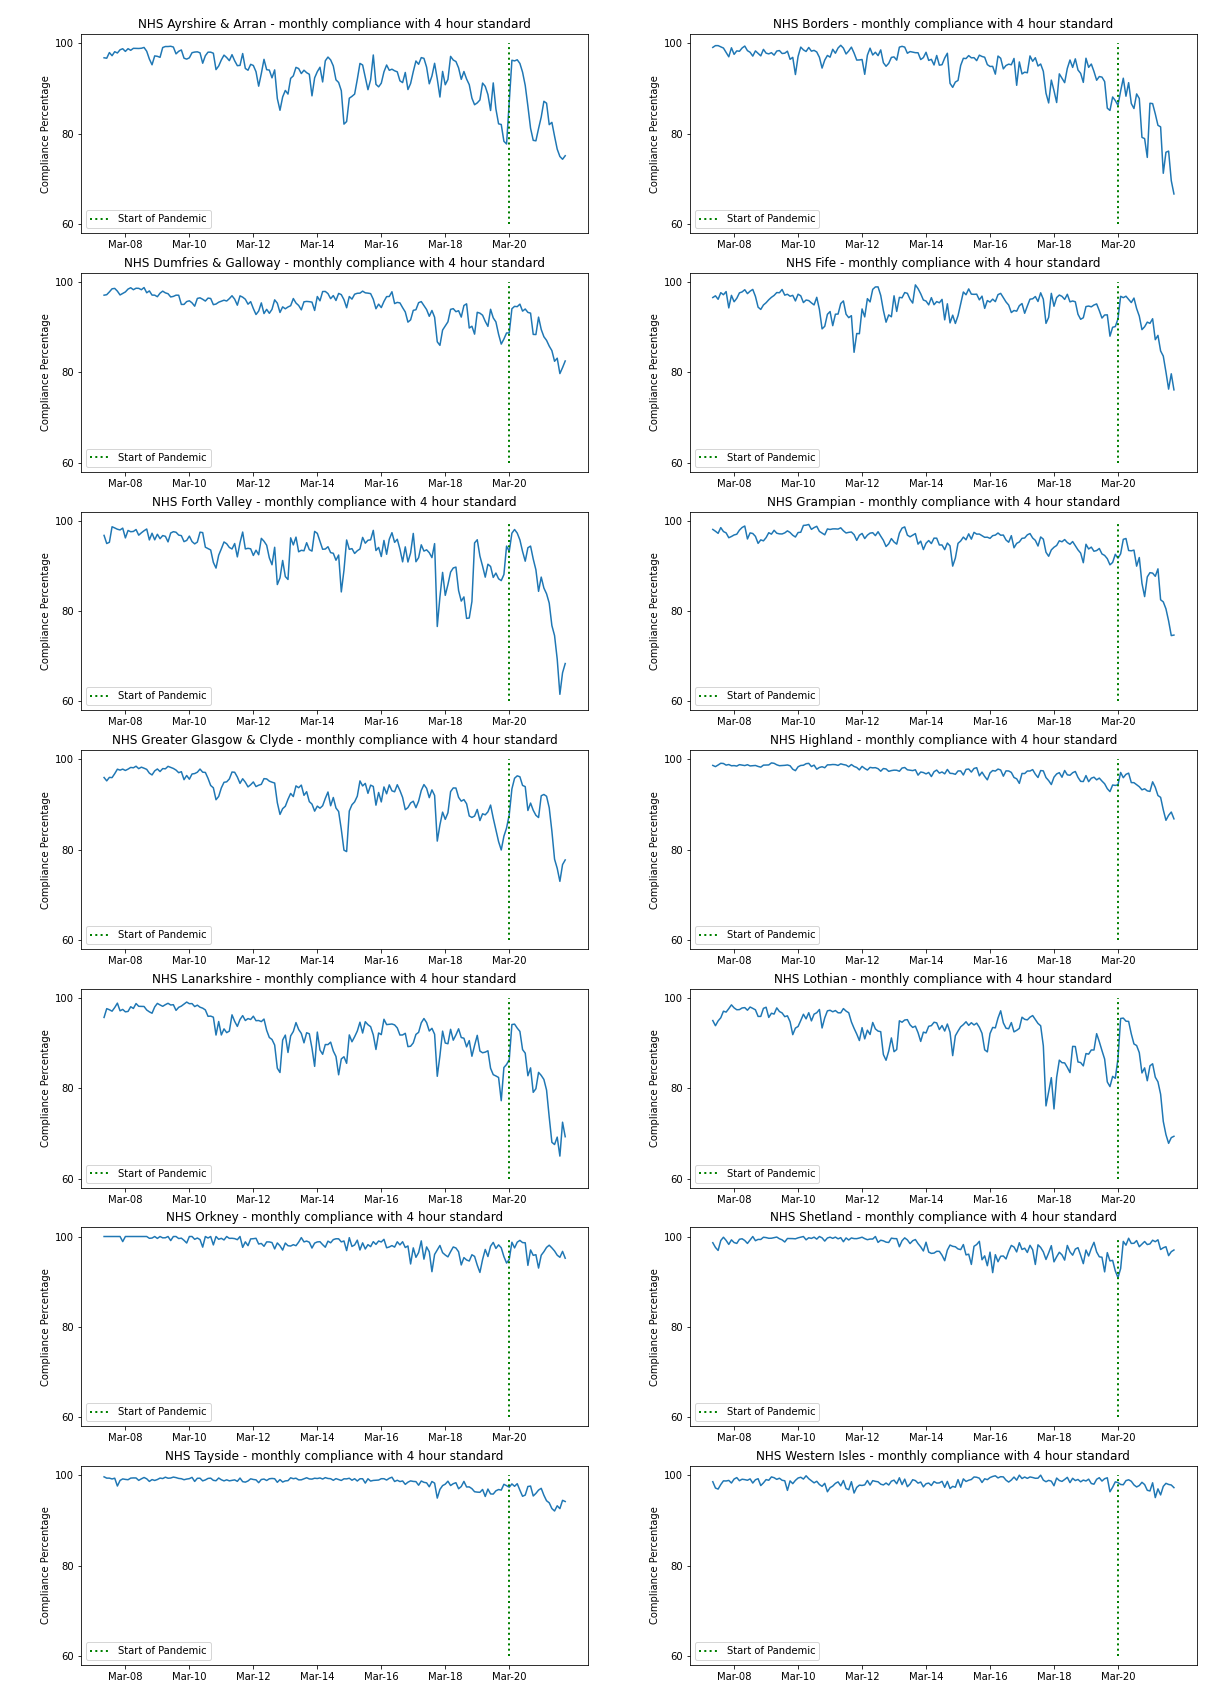
\includegraphics[width=\linewidth]{Monthly_compliance_area_wise.png}
  \caption{Figure showing change in compliance of different regions }
\end{figure}

\newpage
\printbibliography
\end{document}